\chapter{Minecraft as a Simulation Environment for MicroPsi 2}
The objective of this project is to build and test an interface in between MicroPsi and Minecraft, so that a Minecraft world (e.g. server) can be used as a simulation environment for the MicroPsi 2 Framework, which will act as an artificial player.

The modular architecture of MicroPsi 2 allows it to add new simulation environments (or worlds, as they are called in MicroPsi) fairly easily. A world needs interfaces to Data Sources and Data Targets and to a step-function that evolves the world and is being called frequently by the MicroPsi core. These interfaces are provided by the so called world adapter. 

On the other hand, communication with a Minecraft Server typically requires a constant flow of data packets going in and out. Most third party clients, including Bots, facilitate own event loops. 

    \section{Using Spock as the interface in between MicroPsi and a Minecraft server}
The strategy is to add a ``Minecraft'' world to MicroPsi. However, the simulation of the world itself, does not take place in MicroPsi itself, but on a regular Minecraft Server. Instead, Spock is integrated into MicroPsi and incarnates the world. It communicates with the Minecraft server via the Client-Server-Protocol and provides data sources and targets to the world adapter. That way, to MicroPsi it looks like spock is the simulation environment itself, where in fact it's just the interface to game world server.

For this project, the event loop of the bot framework had to be dissolved and rebuilt as the step function of the MicroPsi world. It should be noted, that the frequency in which the framework steps the bot has to be at least chosen so, that it is able to send keep-alive-signals to Server, to not get kicked from the server.

That being said, a big part of the project is about visualization. Inside the MicroPsi Core Application, a 3D-visualization of the Minecraft world and the agent within is generated. There are two main reasons for this. The first reason is, that the agents behavior within the simulation environment is supposed to be visually monitored from the MicroPsi webinterface. The second reason is, that the image data is supposed to be processed by the agent as one of it's ``senses''.

At the same time, the visualisation component reads from Spock's internal gameworld representation to generate a 3D model of the agent's environment. Specifically, the representation of a chunk is fetched and for every solid cube in this chunk, in the visualisation a cube is rendered with Pyglet's OpenGL abstraction. Each block gets it's own textures according to it's type. It is compatible to the widely available Minecraft texture packs. The resulting image is exported as a JPEG file and constantly refreshed in the web interface.

THIS IS WHAT THE MINECRAFT WORLD ADAPTER IS DOING:
FIRST spinning up bot

\begin{figure}[ht]
			\centering
			\begin{minipage}{11cm}
				\begin{pseudocode}
			self.client = Spock(plugins=plugins)
            self.client.start()
            vis.commence_vis(self.client)
            self.first_step = False
				\end{pseudocode}
				\caption{Sending a packet that moves the agent on block in x direction}
				\label{snippet_position-packet}
			\end{minipage}
		\end{figure}
		
SECOND read world data and fill data sources

\begin{figure}[ht]
			\centering
			\begin{minipage}{11cm}
				\begin{pseudocode}
			x_coord = self.world.client.position['x'] * -1
			self.datasources['x_coord'] = x_coord
				\end{pseudocode}
				\caption{Sending a packet that moves the agent on block in x direction}
				\label{snippet_position-packet}
			\end{minipage}
		\end{figure}

THIRD fill datatargets

\begin{figure}[ht]
			\centering
			\begin{minipage}{11cm}
				\begin{pseudocode}
self.datatargets['diamond_offset'] = diamond_coords[0]
				\end{pseudocode}
				\caption{Sending a packet that moves the agent on block in x direction}
				\label{snippet_position-packet}
			\end{minipage}
		\end{figure}
		
FOURTH repeat

INSIDE SPOCK, THIS IS WHAT HAPPENS:

FIRST it's step method is called by the MicroPsi runtime. by default it's maintaining standard communication with the Minecraft Server.

\begin{figure}[ht]
			\centering
			\begin{minipage}{11cm}
				\begin{pseudocode}
self.datatargets['diamond_offset'] = diamond_coords[0]
				\end{pseudocode}
				\caption{Sending a packet that moves the agent on block in x direction}
				\label{snippet_position-packet}
			\end{minipage}
		\end{figure}

... result: a Minecraft Bot that implements MicroPsi AI and is controlled and monitored via the MicroPsi webinterface ...
... the Webinterface holds its own visualization of the Agents worldview ...

To make the bot work as a simulation world, two main challenges had to be overcome. First, the event loop and handling of spock had to be modified to work with MicroPsi. Therefore, the functions that were usually called from within the event-loop now have to be called from within the step function of the world-adapter. The same holds for event handling. 

Second, a system for communicating "sensory data" and commands in between the bot (or Minecraft world) and the world adapter had to be implemented. Up to a certain degree, spocks plug-in system could be facilitated (well ...). In most/ cases, though, sending commands and receiving data (...) had to be be implemented on packet level.

Sending packets in spock is fairly easy. (see figure \ref{snippet_position-packet}

\begin{figure}[ht]
			\centering
			\begin{minipage}{11cm}
				\begin{pseudocode}
					'x': (client.position['x'] + 1)  / 1,
    					'y': client.position['y'] / 1,
					'z': client.position['z'] / 1,
					'on_ground': False,
					'stance': client.position['y'] + 0.11
					}))
				\end{pseudocode}
				\caption{Sending a packet that moves the agent on block in x direction}
				\label{snippet_position-packet}
			\end{minipage}
		\end{figure}
		
%TODO code example fails to latex compile with //

%TODO remove well ...

%explain spocks plugin system
... spocks plugin system ...
%TODO describe, why the bot is "the world"

The worldadapter spins-up and steps a spockbot as follows:

\begin{figure}[ht]
			\centering
			\begin{minipage}{11cm}
				\begin{pseudocode}
    def step(self):
        if self.first_step: #TODO probably not too smart
            # launch minecraft bot
            plugins = [DebugPlugin.DebugPlugin, ChatMessage.ChatMessagePlugin, ChunkSaver.ChunkSaverPlugin] #TODO not all plugins - if any - are needed
            self.client = Client(plugins=plugins)
            self.client.start()
            vis.commence_vis(self.client)
            self.first_step = False

        self.chat_ping_counter += 1
        if self.chat_ping_counter % 100 == 0: #TODO find other way to send "keepalive"
            self.client.push(Packet(ident = 0x03, data = {
						'text': "I'm alive! ping %s" % (self.chat_ping_counter) }))
        World.step(self)
        self.client.step()
        vis.step_vis()
				\end{pseudocode}
				\caption{The MicroPsi world-adapter spins up and steps a spock bot}
				\label{snippet_position-packet}
			\end{minipage}
		\end{figure}
		
Inside spock this looks like this:

\begin{figure}[ht]
			\centering
			\begin{minipage}{11cm}
				\begin{pseudocode}

				\end{pseudocode}
				\caption{The MicroPsi world-adapter spins up and steps a spock bot}
				\label{snippet_position-packet}
			\end{minipage}
		\end{figure}

\paragraph{Data Targets and sources}


    \section{The Visualisation component}
Early ideation made it clear, that this project should contain a visualization component. 

The visualization is supposed to serve two causes. First, it should make it effective and pleasurable to monitor the bot's behavior as well as the environment it is behaving in. Second, it is supposed to serve the agent as a datasource itself. This means, that from pure world data (what block sits where) a 3D-visualization has to be generated from within the MicroPsi Python Code. It should contain a perspective that gives a good overview over the bots environment to forward to the webinterface, as well as a first person perspective of the agent, to function as its eyes.

As the open-source game, which has been used to implement the visualization, uses the graphics and game library pyglet (that basically encapsulates PyOpenGL), which brings it's own event-loop and -handling, the event-loop had to by broken apart and rebuilt as a part of the world adapter (that advances the visualization with every step) .

%TODO define pyglet

\paragraph{monitoring the bot from the webinterface}
... make it aesthetically appealing as well as easily accessible ...

\paragraph{using visualization output as a Datasource / as the bots eyes}

\subsubsection{Implementation}

It has been implemented as follows:

\paragraph{used Data}
... required Data for the visualization ...
... and how to obtain it (first attempts: telnets/then sockets) ...

\subsubsection{3D Visualisierung mit Pyglet}
Fortunately, a (Minecraft inspired) open source (MIT license) project has been found, that implements a (very) simple Minecraft clone in (under 500 lines of) Python.\cite{github_minecraftpython}

The code of this project could be facilitated to serve as a visualization.
... additional 3D models, blocks an graphics had to be added ...

\subsubsection{Earlier attempts using JavaScript / AJAX}
... worked well but a little slow ...

\section{A! Implementation}

Viewing the resulting software as a whole, several modules have been added to the architecture: the Minecraft world adapter, the spock bot (communicating with a Minecraft Server) and the (pyglet) Visualization. (see figure \ref{uml_mc})

\begin{figure}[h]
  \centering
    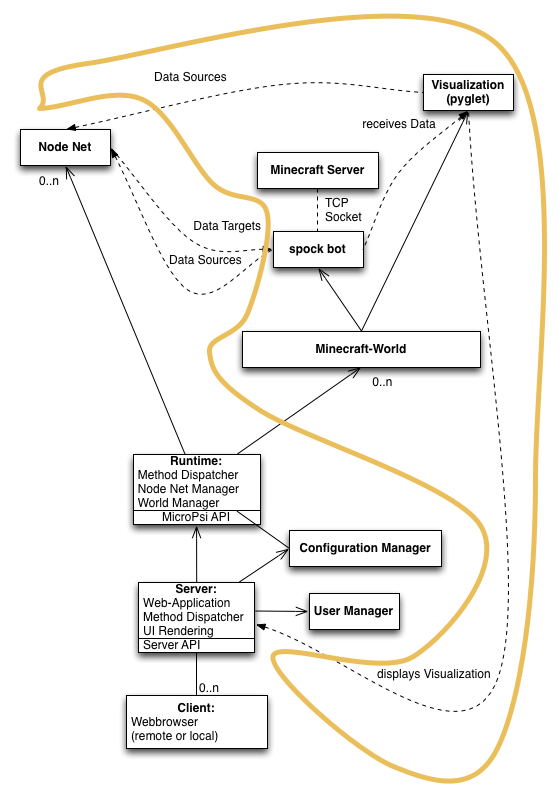
\includegraphics[width=10cm]{graphics/UML_MicroPsi_mit_spock_und_rahmen}
  \caption{The new architecture of MicroPsi with the Minecraft interface. New modules are framed orange.}
  \label{uml_mc}
\end{figure}

... graphic/UML of the project as a whole ...
... illustration of the event loop ...

% TODO je nach Größe des Kapitels, das hier vielleicht eine Ebene höher ziehen (versuche dich hier erstmal nur auf die fertige Lösung zu konzentrieren und warum du dich dafür entschieden hast. Es ist nicht interessant, was du sonst alles ausprobiert hast, außer dass du konkret angibst, warum du dich für die jetztige Implementierung im Vergleich zu anderen entschieden hast)

\section{A! Case Study}

The functionality is to be tested with a simple Braitenberg-vehicle experiment.

\subsection{Experiment}
... experiment to test functionality of the system ...
... scope: only a simple test for time reasons ...

\subsubsection{Braitenberg Vehicle}
... simplest proof of concept of a microPsi agent ...